\documentclass[notitlepage]{report}

\title{
	\textsc{ \small
		Physics 415
	} \\
	{\textsc{\small Lab \#4}} \\
	Gaussian beam measurement
}
\author{Kevin Evans \\ Partner: Sierra Ray}
\date{March 18, 2021}
\usepackage{amssymb}
\usepackage{mathtools}

\usepackage{amsthm}
\usepackage{amsmath}
\usepackage{slashed}
\usepackage{relsize}
\usepackage{threeparttable}
\usepackage{float}
\usepackage{booktabs}
\usepackage{boldline}
\usepackage{changepage}
\usepackage{physics}
\usepackage[inter-unit-product =\cdot]{siunitx}
\usepackage{setspace}
\usepackage{caption}
\usepackage{subcaption}
\usepackage[makeroom]{cancel}
%\usepackage{pgfplots}
%\usepackage{pdfpages}
\usepackage[hidelinks]{hyperref}
\usepackage{enumitem}
\usepackage{times}
\usepackage{titling} % for titlingpage environment
\usepackage{calligra}
\usepackage{graphicx}
\DeclareMathAlphabet{\mathcalligra}{T1}{calligra}{m}{n}
\DeclareFontShape{T1}{calligra}{m}{n}{<->s*[2.2]callig15}{}
\newcommand{\scriptr}{\mathcalligra{r}\,}
\newcommand{\boldscriptr}{\pmb{\mathcalligra{r}}\,}
\newcommand{\emf}{\mathcal{E}}
\renewcommand{\thesection}{\arabic{section}}

\begin{document}
	\begin{titlingpage}
		\maketitle
		\begin{abstract}
			\noindent 
			The relative intensity of the HeNe passing through a polarizer was measured as a function of polarizer angle. This showed nonlinear behavior at high intensities as the photodiode saturates. In the subsequent experiments, a polarizer was placed at \SI{45}{\deg}, halving the intensity to a linear region on the photodiode.
			
			The beam profile of the HeNe laser was measured using a knife edge on a translation stage. This was done by slowly incrementing the translation stage perpendicular to the beam, ranging from all light passing through to blocking the light fully. The data was plotted in Origin and a curve fit was applied using an $\mathrm{erfc}$ function. This resulted in a beam width of $\SI{0.399}{\mm} \pm \SI{0.11}{\mm}$ at a location $\SI{21.9}{\centi\meter}$ from the laser shutter.
			
			The beam profile was additionally measured using the ``70-30'' technique. This was done by finding the relative maximum and minimum intensity, then calculating the $0.30$ and $0.70$ intensities. At several points along the beam axis, the translation distances was measured for these two intensities. The data was plotted in Origin and a curve fit was applied using a Gaussian width function.
			
			The HeNe laser was profiled to have a beam waist $w_0=\SI{0.275}{\mm} \pm \SI{16.1}{\um}$, located at the focus $z_0 = -\SI{12.1}{\centi\meter} \pm \SI{12.0}{\centi\meter}$ relative to the HeNe laser, i.e. located within the laser.
		\end{abstract}
	\end{titlingpage}

	\section{Description of Experiment}
	In this experiment, we will measure the beam profile of the HeNe laser using a knife edge. To begin, we will verify the powermeter gives a linear reading. This is accomplished by placing a polarizer between the laser and the powermeter wand, then profiling the intensity as a function of the polarizer angle. This data was plotted in Origin with a sinuosodial curve fit. As the powermeter saturates, the polarizer was later used to reduce the intensity to a linear region of the powermeter readings. 
	
	Next, a knife edge was mounted on a translation stage perpindicular to the laser beam. The stage was mounted \SI{21.9}{\centi\meter} from the shutter of the laser. The translation stage was slowly adjusted from allowing the laser to pass to completely blocking the incident light to the powermeter. The corresponding intensity measurements were recorded and plotted in Origin as a function of the translation distance. The fit function used is given by \begin{equation}
		P  = P_0 + \frac{ P_\mathrm{max} }{2} \mathrm{erfc}\left(\frac{\sqrt{2}(x-x_0)}{w}\right) \label{eq:erf}
	\end{equation}
	where the measured voltage is proportional to the power $P$, and $w$ is the waist radius at the distance chosen.
	
	Then, the ``70-30'' technique was employed to measure the beam waist. This was done by using the maximum intensity of the light and multiplying by $0.30$ and $0.70$. At various points along the beam, the distance from the laser was recorded, as well as the translation distance at the two intensities. Mirrors were used to redirect the beam, keeping the beam within the optical breadboard. The data was recorded in Origin and a non-linear curve fit was applied using \begin{equation}
		w(z) = w_0 \sqrt{1 + \frac{ \lambda^2 (z-z_0)^2 }{\pi^2 {w_0}^2} } \label{eq:width}
	\end{equation}
	From the curve fit, the beam waist $w_0$ and true origin of the beam $z_0$ was found. 
	
	\section{Data and Analysis}
	With the laser blocked, the powermeter reading was \SI{281.2}{\mV} from the ambient light. The polarizer was then placed between the laser and powermeter. This data was recorded and plotted in Origin, shown in Figure \ref{fig:lab4polarizer}. The resultant fit is poor, due to the nonlinearity of the power meter at high intensities. Because of this, the polarizer was kept at \SI{45.0}{\deg}, resulting in a new minimum of \SI{278.9}{\mV} and maximum of \SI{339.8}{\mV}.
	
	\begin{figure}[p]
		\centering
		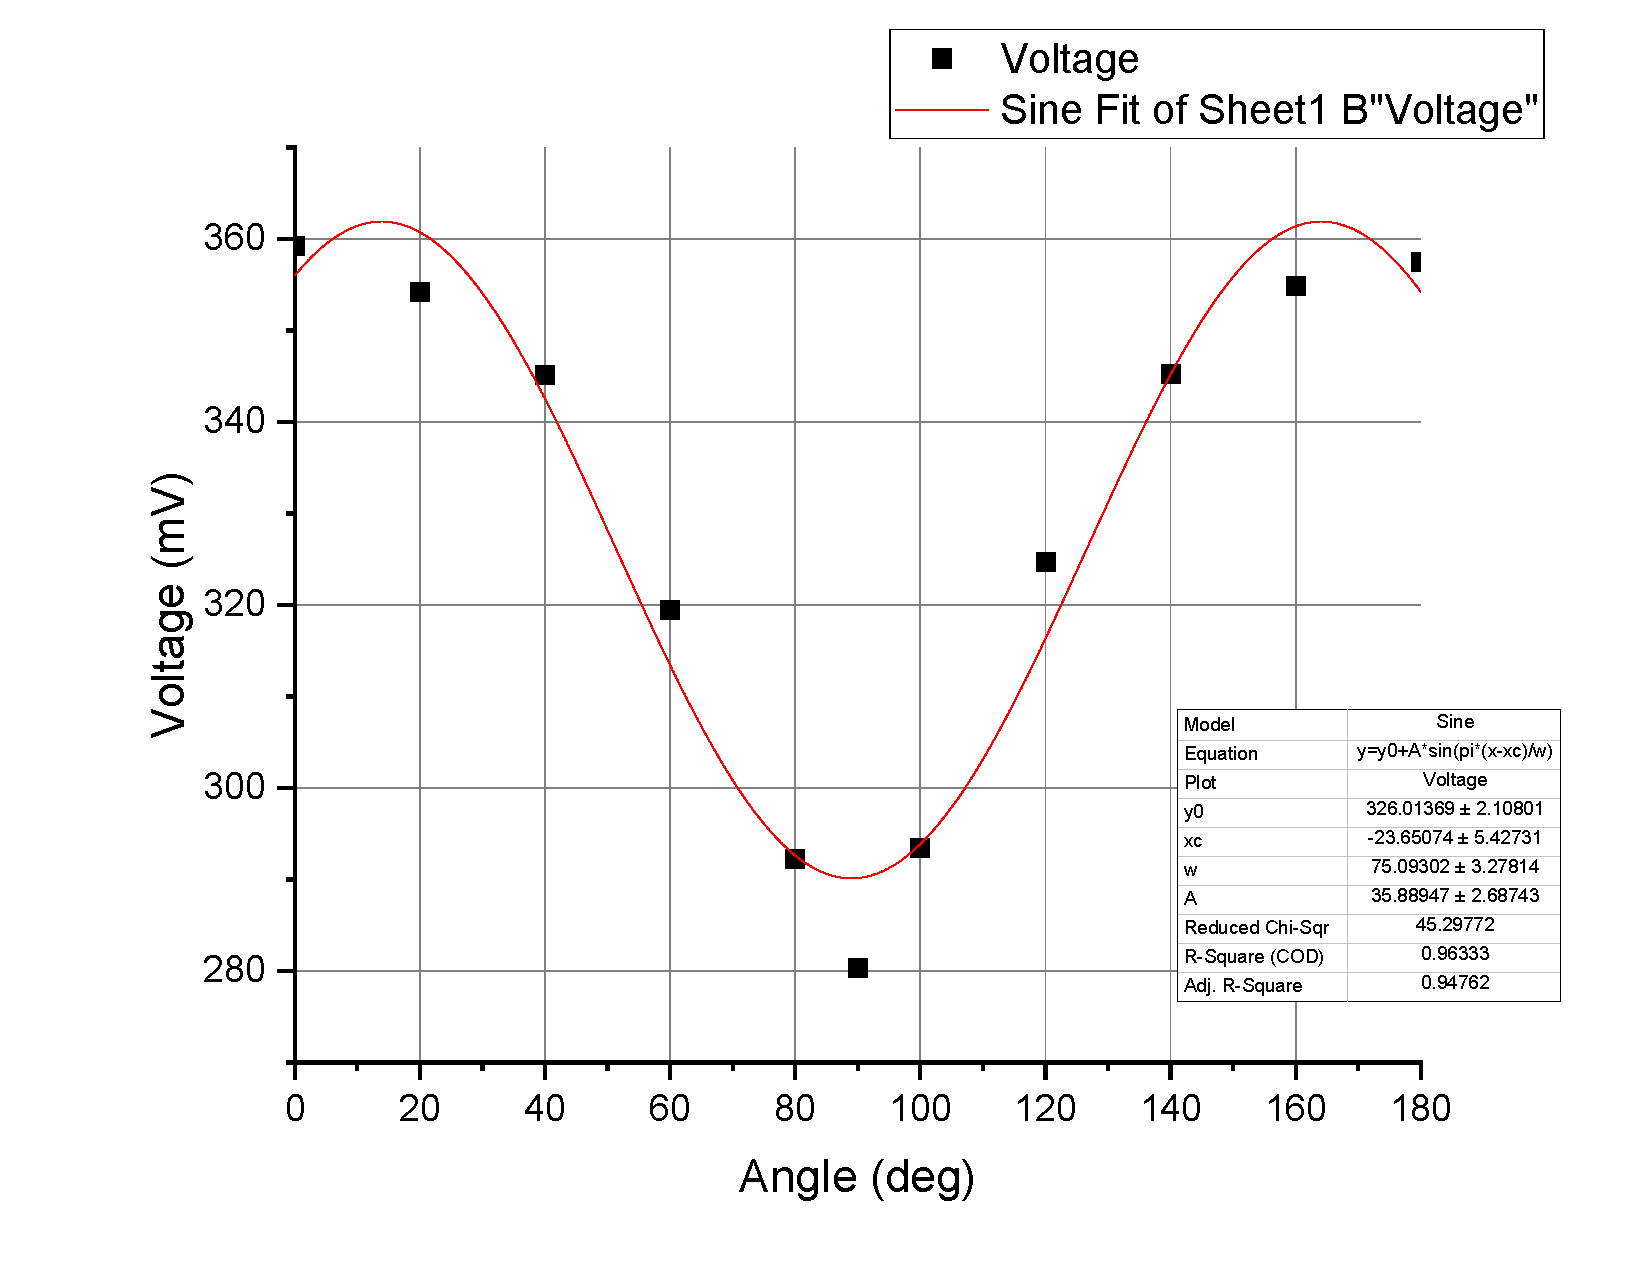
\includegraphics[width=0.7\linewidth]{lab4_polarizer}
		\caption{The relative intensity as a function of angle. The poor fit is likely due to clipping near the higher intensities caused by the photodiode saturating.}
		\label{fig:lab4polarizer}
	\end{figure}

	
\begin{figure}[p]
	\centering
	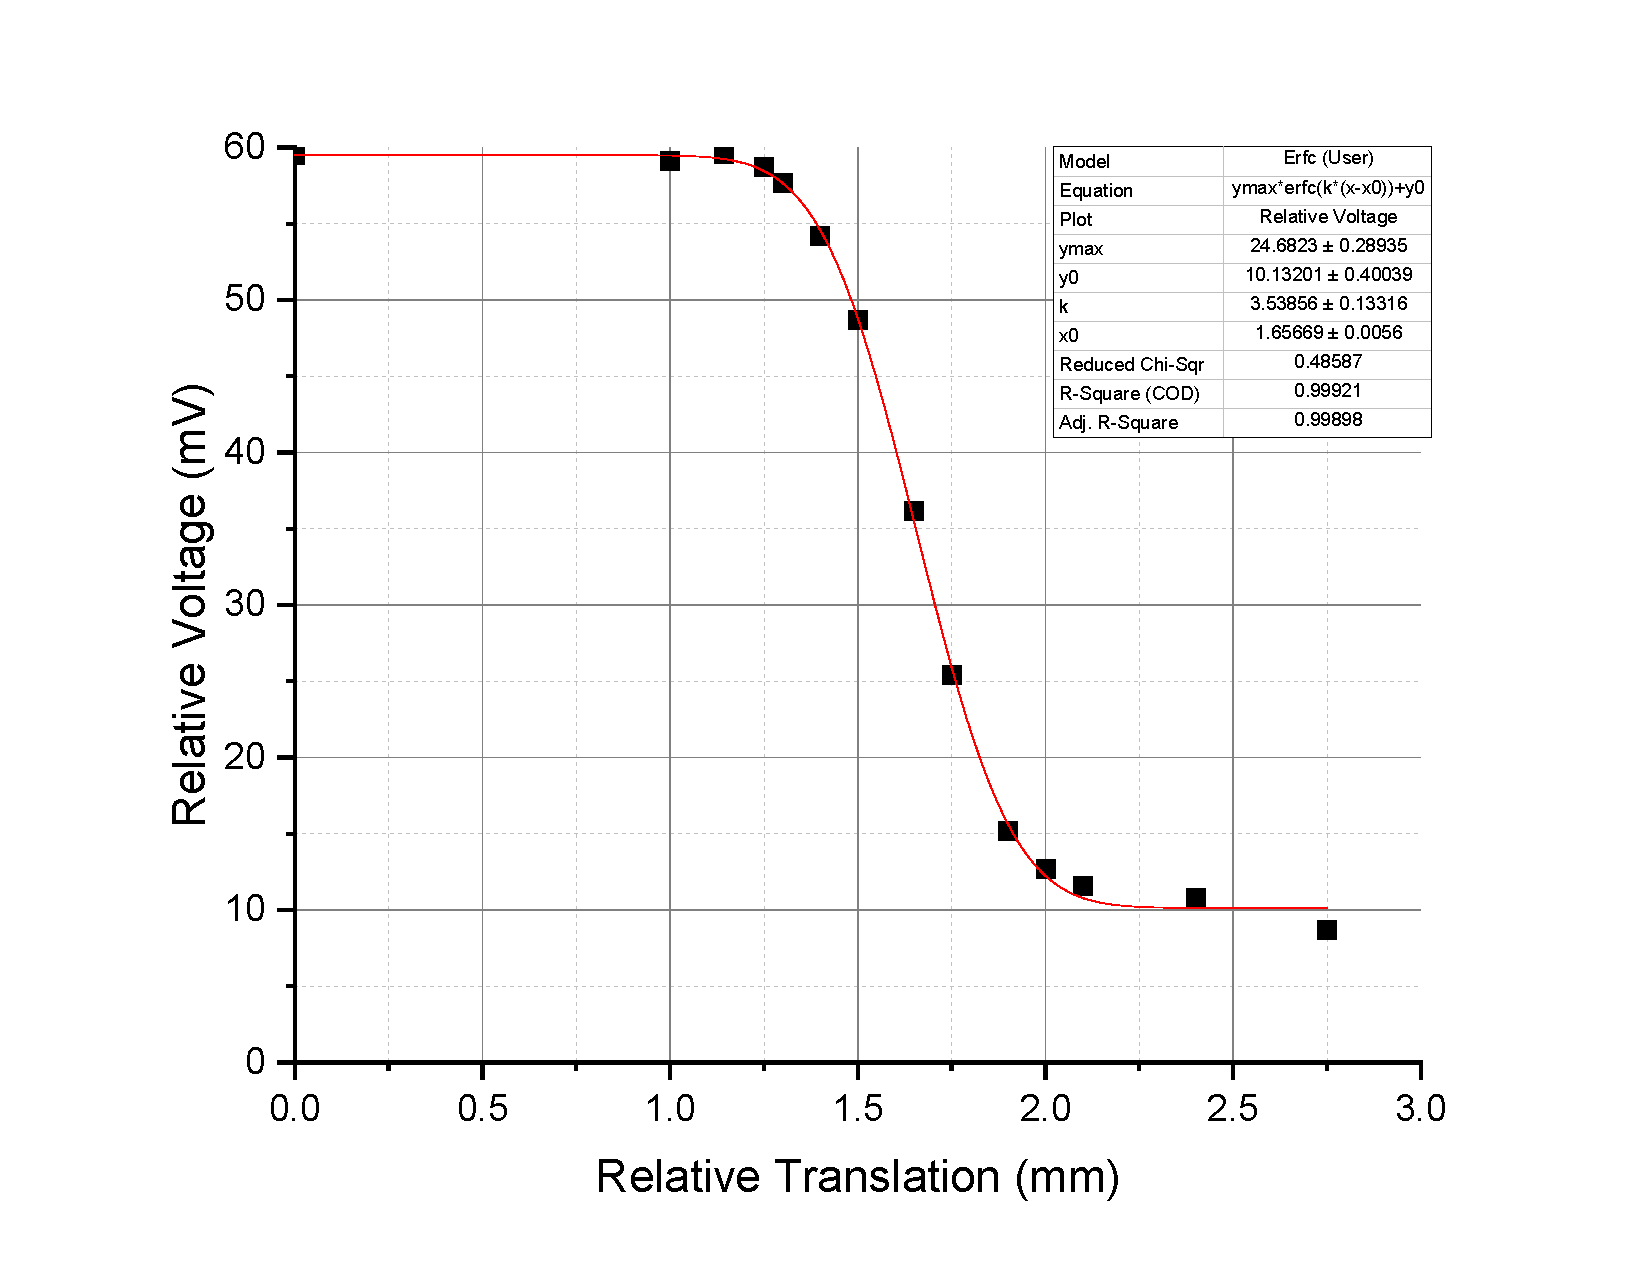
\includegraphics[width=0.9\linewidth]{lab4_erfc}
	\caption{The beam intensity profile as a function of translation distance.}
	\label{fig:lab4erfc}
\end{figure}	
	
	\subsubsection{Fixed point profile measurements}
	The profile was measured as a function of translation distance of the knife edge at a distance $z=\SI{21.9}{\centi\meter \pm \SI{0.1}{\centi\meter}}$ from the laser shutter. This data is shown in Figure \ref{fig:lab4erfc}, with the curve fit of form \eqref{eq:erf} applied. The curve fit results in a width $w=\SI{0.399}{\mm}$.

	
	
	\subsubsection{Beam profile measurements using 30-70 technique}
	
	The distance $z$ was measured with $\pm 1$ inch (\SI{\pm 2.54}{\centi\meter}) accuracy using the optical breadboard grid, then using a ruler to measure the offsets relative to the threaded hole. This was plotted and shown in Figure \ref{fig:lab4thing}. Applying \eqref{eq:width}, the beam waist $w_0=\SI{0.276}{\mm} \pm \SI{16.1}{\um}$, with the focus at $z_0=\SI{-12.1}{\centi\meter} \pm \SI{12.0}{\centi\meter}$. The uncertainty was calculated using the estimated standard deviation within Origin.
	
	The expected value for the beam waist is roughly \SI{0.33}{\mm}\footnote{From the manufacturer website:
		 \url{https://www.global-optosigma.com/en\_jp/Catalogs/gno/?from=page\&pnoname=05-LHP\&ccode=W5002\&dcode=\&gnoname=05-LHP-991}}, which creates an approximate error of 15.1\%.
	 
	
	
	
	\section{Results and Conclusion}
	The beam was found to have a beam waist of $w_0=\SI{0.276}{\mm} \pm \SI{16.1}{\um}$ with $z_0=\SI{-12.1}{\centi\meter}$. The negative $z_0$ implies the laser cavity is confocal within the laser itself. Compared to the $1/e^2$ radius, there was roughly 15.1\% error, but this error may be due to imprecise ($\pm 1 \text{ in}$) measurements of the distance $z$ and a poor curve fit. 
	
		\begin{figure}[h]
		\centering
		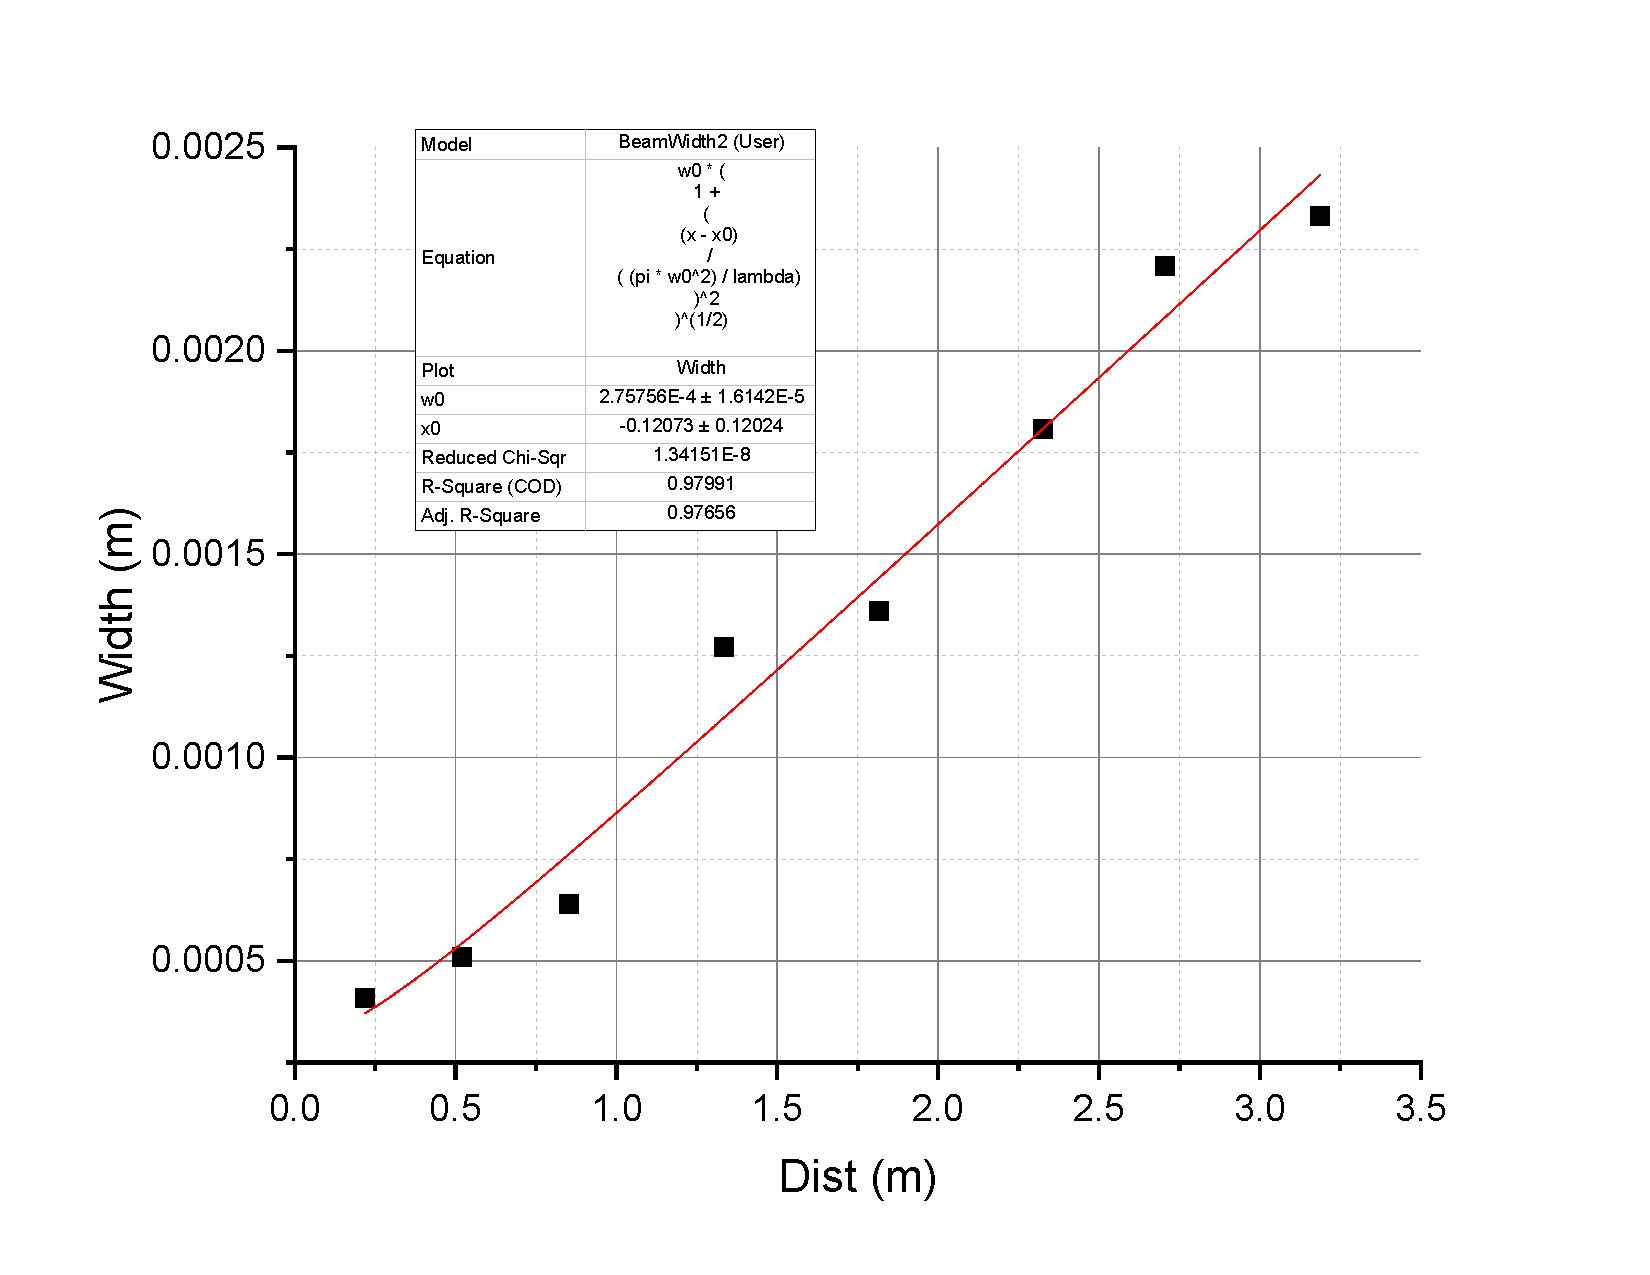
\includegraphics[width=\linewidth]{lab4_thing}
		\caption{The beam waist as a function of distance along the beam axis.}
		\label{fig:lab4thing}
	\end{figure}
	
	\pagebreak
	\section*{Data tables}
	% Please add the following required packages to your document preamble:
	% \usepackage{booktabs}
	\begin{table}[H]
		\centering
		\caption{Intensity as a function of polarizer angle}
		\begin{tabular}{@{}ll@{}}
			\toprule
			Angle (deg) & Voltage (mV) \\ \midrule
			0           & 359.2        \\
			20          & 354.2        \\
			40          & 345.2        \\
			60          & 319.5        \\
			80          & 292.2        \\
			90          & 280.3        \\
			100         & 293.5        \\
			120         & 324.7        \\
			140         & 345.3        \\
			160         & 354.9        \\
			180         & 357.5        \\ \bottomrule
		\end{tabular}
	\end{table}

% Please add the following required packages to your document preamble:
% \usepackage{booktabs}
\begin{table}[H]
	\centering
	\caption{Intensity as a function of translation}
	\begin{tabular}{@{}ll@{}}
		\toprule
		Translation (mm) & Intensity (mV) \\
		\midrule
		20               & 338.4          \\
		19               & 338.0          \\
		18.856           & 338.5          \\
		18.75            & 337.6          \\
		18.7             & 336.6          \\
		18.6             & 333.1          \\
		18.5             & 327.6          \\
		18.35            & 315.1          \\
		18.25            & 304.3          \\
		18.1             & 294.1          \\
		18               & 291.6          \\
		17.9             & 290.5          \\
		17.6             & 289.7          \\
		17.25            & 287.6      \\ \bottomrule   
	\end{tabular}
\end{table}

% Please add the following required packages to your document preamble:
% \usepackage{booktabs}
\begin{table}[H]
	\centering
	\caption{Beam width as a function of distance from HeNe shutter}
\begin{tabular}{@{}ll@{}}
	\toprule
	Distance (cm) & Beam width (mm) \\ \midrule
	21.9          & 0.409           \\
	52.07         & 0.51            \\
	85.09         & 0.64            \\
	133.35        & 1.272           \\
	181.61        & 1.36            \\
	232.41        & 1.809           \\
	270.51        & 2.209           \\
	318.77        & 2.332           \\ \bottomrule
\end{tabular}
\end{table}

	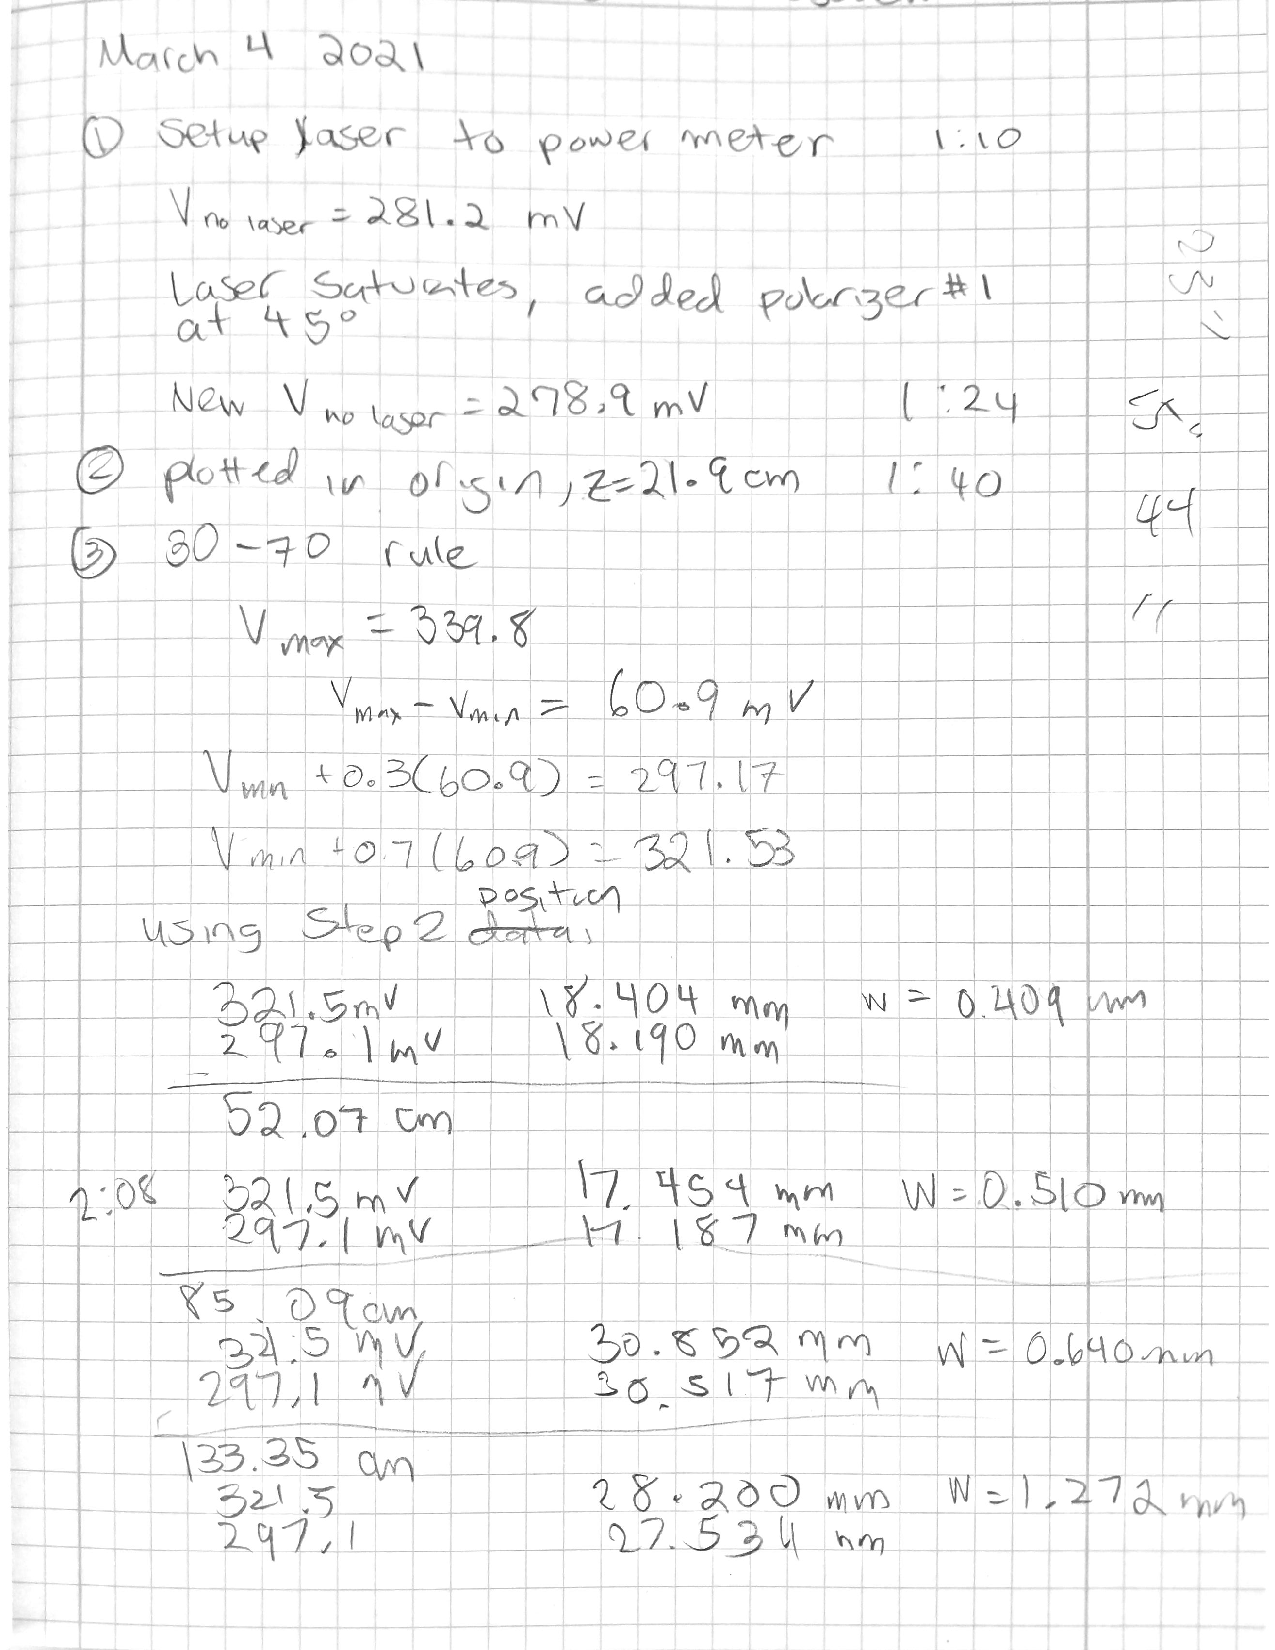
\includegraphics[scale=0.75,page=1]{scanned.pdf}
	
	\includegraphics[scale=0.75,page=2]{scanned.pdf}
\end{document}